\clearpage

\chapter{Use Case Beschreibungen}


\section{Spieler erstellen}
\begin{figure}[!h]
	\centering
    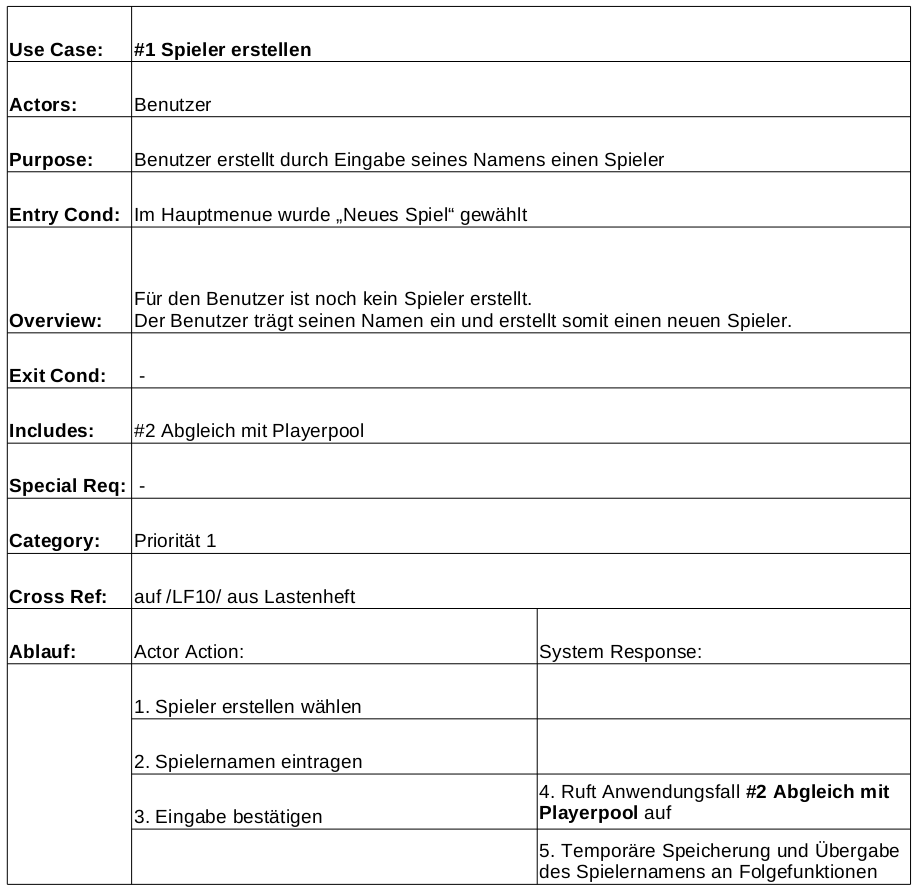
\includegraphics[width=\textwidth]{./ucbSpielerErstellen.png}
	\label{}
\end{figure}

\section{Abgleich mit Playerpool}
\begin{figure}[!h]
	\centering
    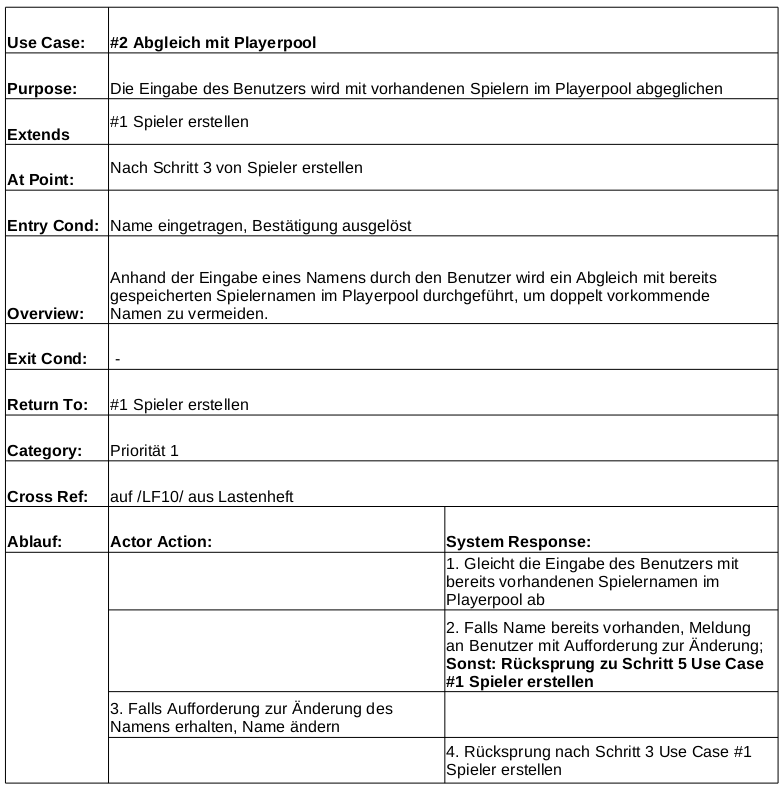
\includegraphics[width=\textwidth]{./ucbAbgleichPlayerpool.png}
	\label{}
\end{figure}


\clearpage
\section{Spieler laden}
\begin{figure}[!h]
	\centering
    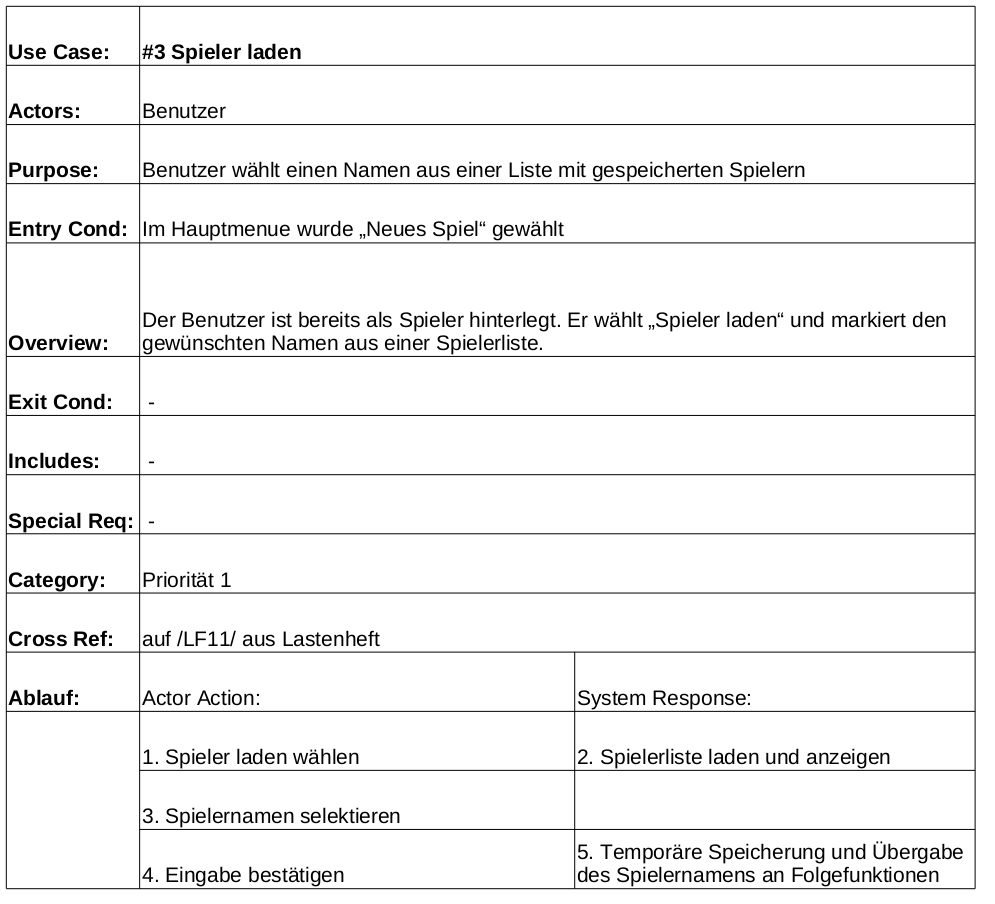
\includegraphics[width=\textwidth]{./ucbSpielerLaden.png}
	\label{}
\end{figure}


\clearpage
\section{Spielmodus wählen}
\begin{figure}[!h]
	\centering
    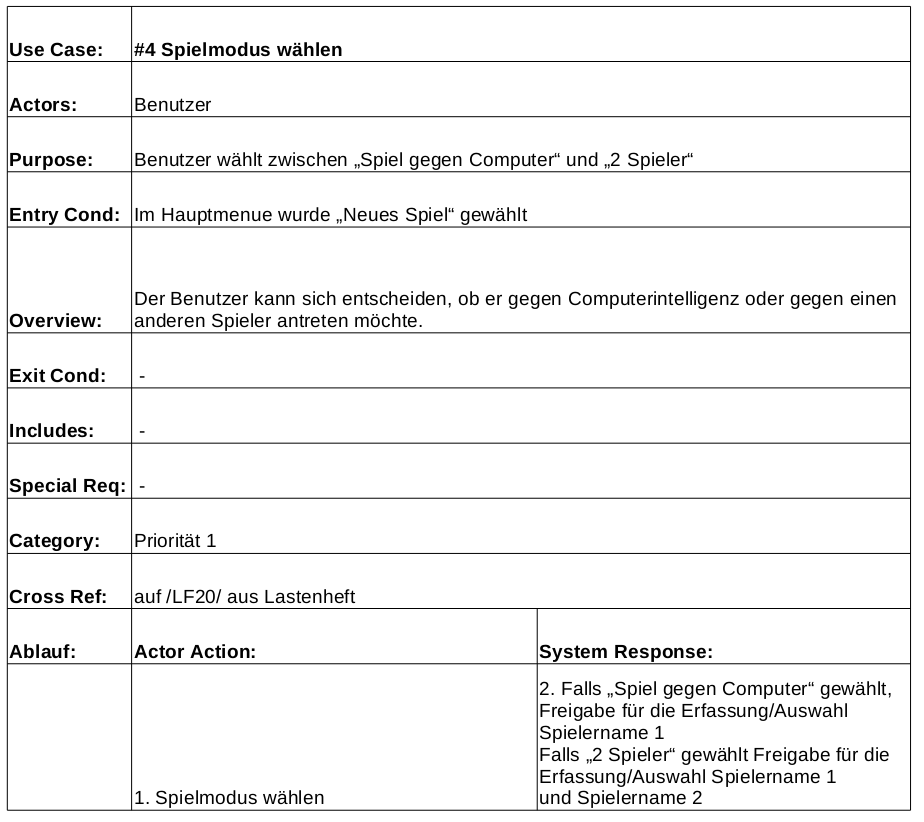
\includegraphics[width=\textwidth]{./ucbSpielmodus.png}
	\label{}
\end{figure}

\clearpage
\section{Thema wählen}
\begin{figure}[!h]
	\centering
    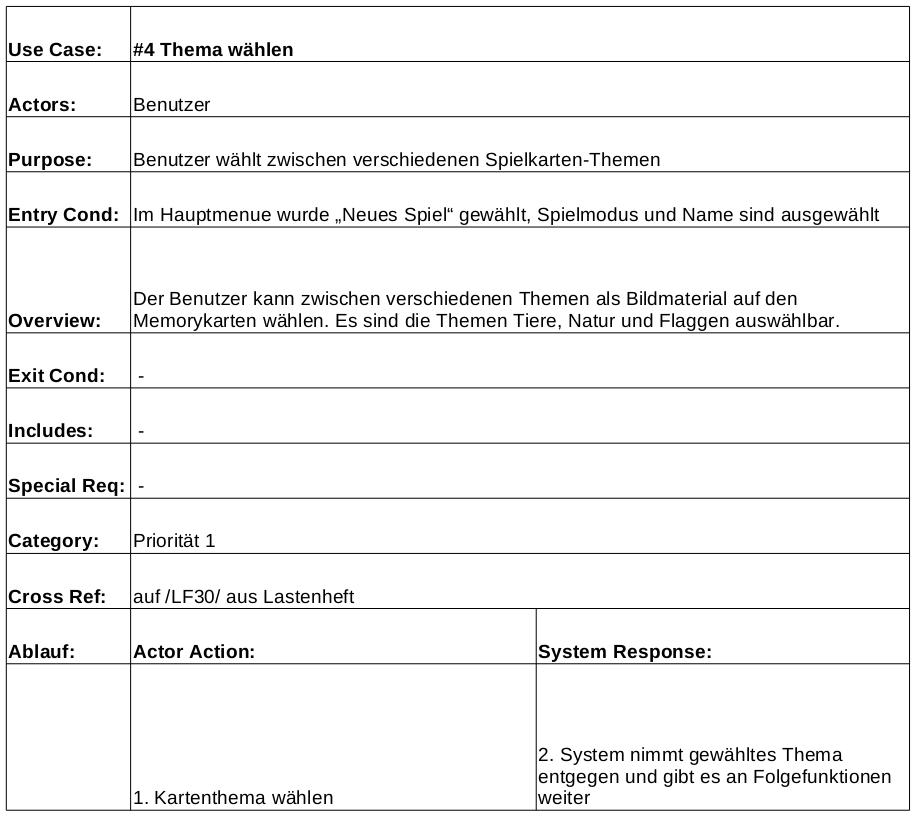
\includegraphics[width=\textwidth]{./ucbThema.png}
	\label{}
\end{figure} 

\clearpage
\section{Spielfeldgröße wählen}
\begin{figure}[!h]
	\centering
    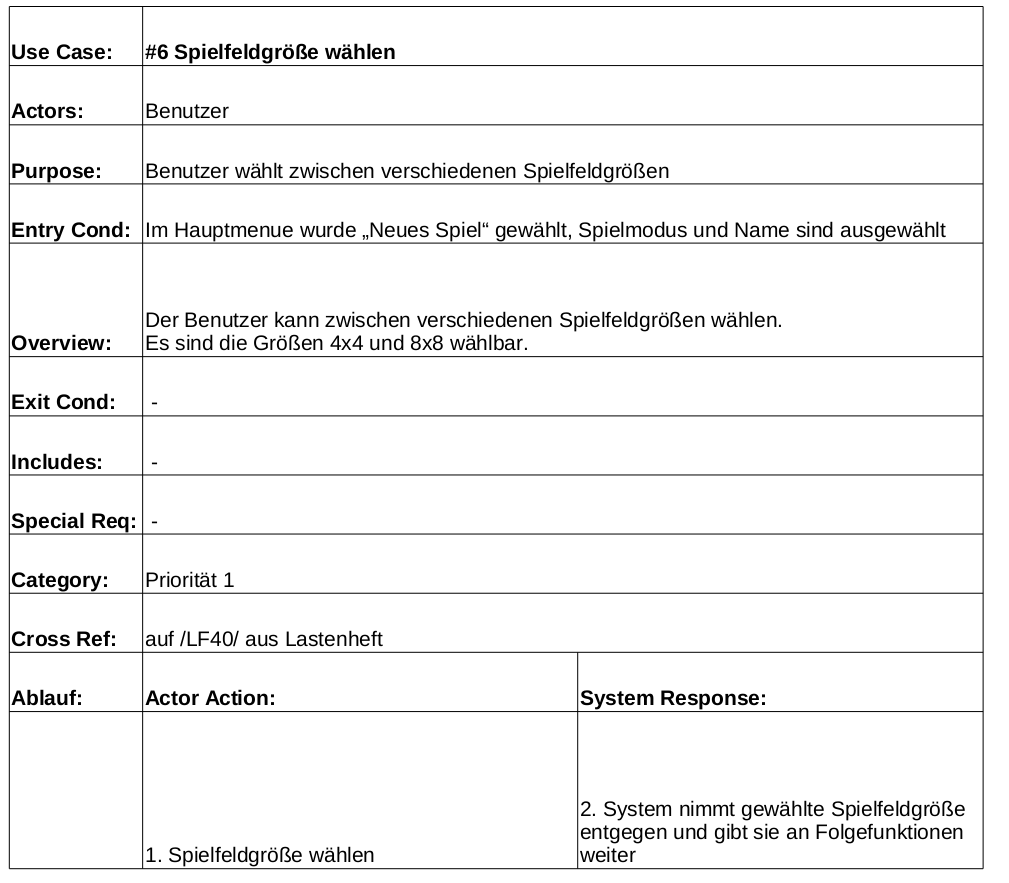
\includegraphics[width=\textwidth]{./ucbSpielfeldgroesse.png}
	\label{}
\end{figure}

\clearpage
\section{Spiel starten}
\begin{figure}[!h]
	\centering
    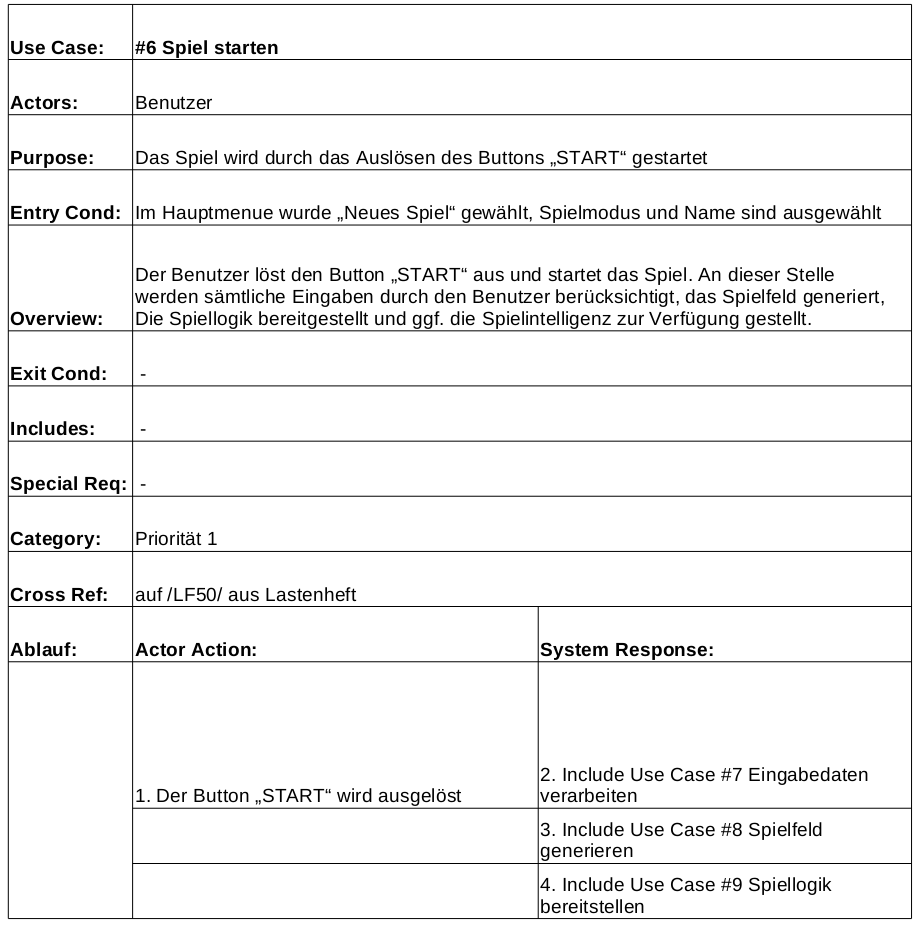
\includegraphics[width=\textwidth]{./ucbSpielStarten.png}
	\label{}
\end{figure}
\paragraph{Bemerkung: }Für die Include Use Cases 7 bis 9 werden keine Use Case Beschreibungen erstellt, weil es sich um Anwendungsfälle handeln, an denen ausschließlich das System beteiligt ist und interne Funktionen aufgerufen werden. Eine detailiertere Darstellung des Use Case ,,Spiel starten`` wird anhand von Sequenzdiagramm und Ablaufdiagramm bereitgestellt.

\clearpage
\section{Highscore anzeigen}
\begin{figure}[!h]
	\centering
    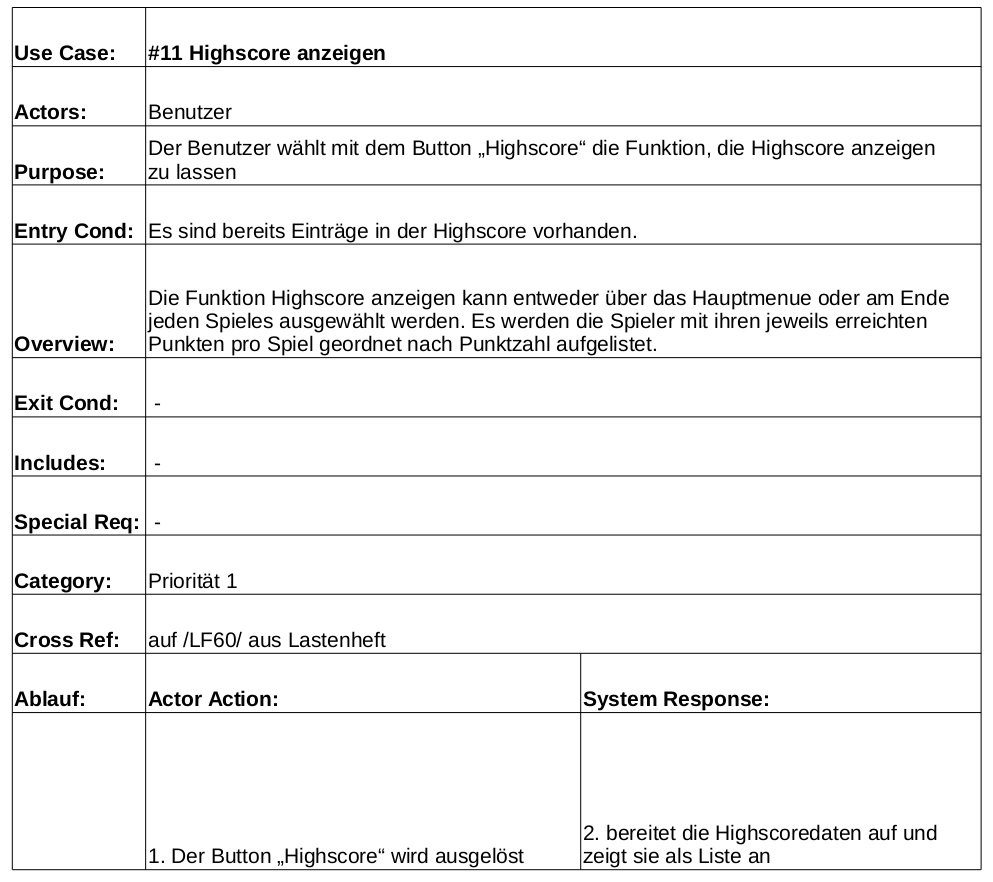
\includegraphics[width=\textwidth]{./ucbHighscore.png}
	\label{}
\end{figure}
